\section{Project Management}

\subsection{Version Control}

Packet Courier was developed using Git\cite{git} as a version control system and the code repository is hosted on
GitHub\cite{github, packet_courier} at \url{https://github.com/thelukethorpe/packet_courier}. There is no special
reason for either of these choices; they are simply industry standards being used for a project that doesn't
innately demand bespoke tooling (unlike data-heavy ventures such as game development, which might benefit from a tool
like Perforce\cite{perforce, perforce_vs_git}).

\subsection{Ticket Tracking}

GitHub Issues\cite{github_issues} powers Packet Courier's ticket tracking. Tickets, or \emph{issues}, as per the
GitHub nomenclature, are categorised based on one or more of the following custom tags:
\begin{itemize}
    \item \textbf{Bug:} \emph{Something isn't working.}
    \item \textbf{CI:} \emph{Change to pipeline.}
    \item \textbf{Documentation:} \emph{Improvements or additions to documentation.}
    \item \textbf{Feature:} \emph{New feature or request.}
    \item \textbf{Optimization:} \emph{Improvements in performance.}
    \item \textbf{Refactor:} \emph{Tech-debt, structural change of quality-of-life improvement.}
    \item \textbf{Testing:} \emph{Improvements or additions to test suite.}
    \item \textbf{Won't Fix:} \emph{This will not be worked on.}
\end{itemize}

Issues are further organised using a Kanban board\cite{kanban_board}. As the \emph{documentation} tag suggests,
this board is not only used for development purposes, in fact, it has been used to help manage the project
holistically, including the writing of this very report, as shown in
Figure~\ref{fig:chapter_4_implementation-github_kanban_board}.

\begin{figure}[!h] {
    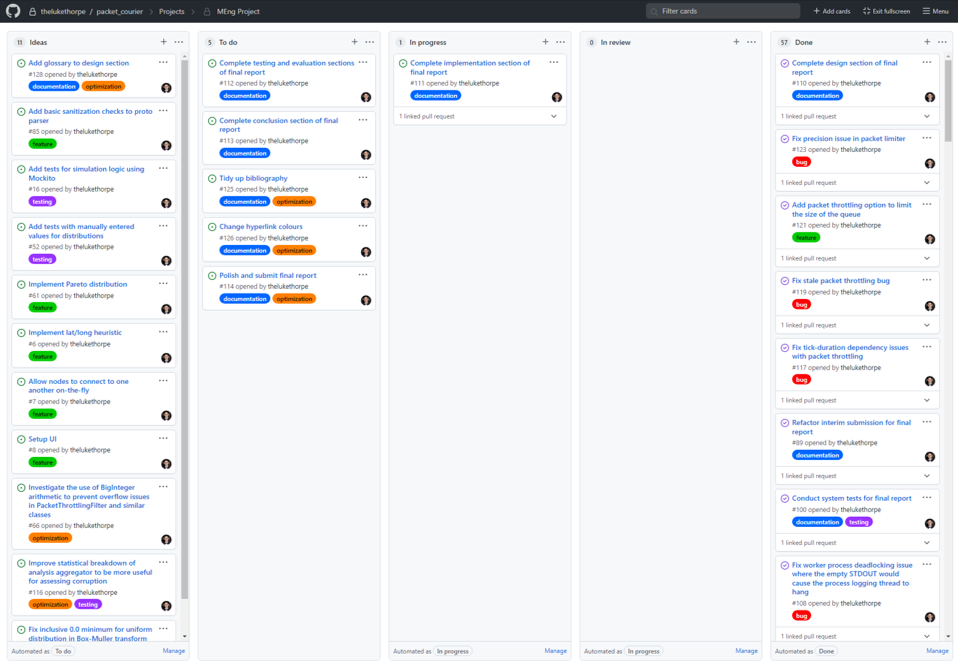
\includegraphics[width=\textwidth]{images/chapter_4_implementation/github_kanban_board}
    \centering~\caption{Packet Courier's Project Kanban Board\cite{packet_courier}.}
    \label{fig:chapter_4_implementation-github_kanban_board}
}
\end{figure}

Pull-requests are opened for every merge to the \texttt{main} branch and linked to the associated ticket number.
Branches are named with a uniform and consistent structure, prefixed by the issue number followed by a brief subtitle
of the ticket delimited by hyphens. Despite being an individual project, this repository has been maintained to
industry standards of software engineering practices for organisational reasons, and has in turn benefited massively
from it.

\begin{figure}[!h] {
    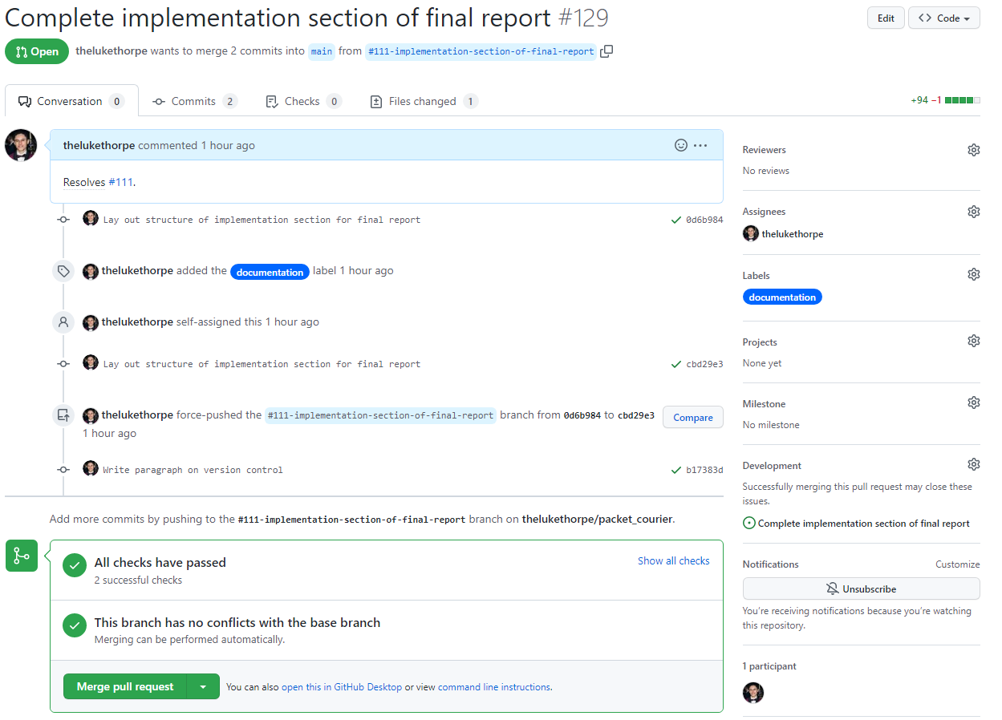
\includegraphics[width=\textwidth]{images/chapter_4_implementation/github_pull_request}
    \centering~\caption{An example of a pull-request in the Packet Courier repository\cite{packet_courier}.}
    \label{fig:chapter_4_implementation-github_pull_request}
}
\end{figure}

\newpage

\subsection{Programming Languages}

TODO

\subsection{Build Management and Dependencies}

\subsubsection{JUnit 4}

TODO

\subsubsection{AssertJ}

TODO

\subsubsection{Google Protobuf}

TODO

\subsubsection{Protocol Buffers Protobuf Maven Plugin}

TODO

\subsection{Continuous Integration}

TODO


\section{API Overview}

\subsection{Repository Structure}

TODO

\subsection{Probability Distribution API}

TODO

\subsection{Network Condition API}

TODO

\subsection{Worker API}

TODO

\subsection{Node API}

TODO

\subsection{Mail API}

TODO

\subsection{Simulation API}

TODO

\subsection{Miscilaneous}

TODO


\section{Standalone Emulator}

\subsection{Key Components}

TODO

\subsection{Protobuf Integration}

TODO


\section{Debugging Features}

\subsection{Process Monitor}

TODO

\subsection{Crash Dumps}

TODO

\subsection{Meta Logging}

TODO
